\documentclass[tikz,border=16pt]{standalone}
\usepackage[utf8]{inputenc}
\usepackage[T1]{fontenc}
\usepackage{lmodern}
\usepackage{xcolor}
\usepackage{tikz}
\usetikzlibrary{positioning, shapes.multipart, arrows.meta, calc, shadows}

% Paleta editorial do projeto (ECOX14 / UNIFEI)
\definecolor{navy}{HTML}{0B2545}
\definecolor{teal}{HTML}{00796B}
\definecolor{teallight}{HTML}{F0FDFA}
\definecolor{amber}{HTML}{B45309}
\definecolor{amberlight}{HTML}{FFFBEB}
\definecolor{slate}{HTML}{334155}
\definecolor{bordergray}{HTML}{CBD5E1}

\tikzset{
  dimbox/.style={
    rectangle split,
    rectangle split parts=2,
    draw=teal,
    line width=1.1pt,
    rounded corners=4pt,
    rectangle split part fill={teal, teallight},
    text width=6.0cm,
    align=left,
    font=\sffamily\footnotesize,
    drop shadow={opacity=0.10, shadow xshift=1.5pt, shadow yshift=-1.5pt},
    inner sep=6pt
  },
  factbox/.style={
    rectangle split,
    rectangle split parts=2,
    draw=navy,
    line width=1.3pt,
    rounded corners=4pt,
    rectangle split part fill={navy, white},
    text width=6.6cm,
    align=left,
    font=\sffamily\footnotesize,
    drop shadow={opacity=0.12, shadow xshift=1.5pt, shadow yshift=-1.5pt},
    inner sep=6pt
  },
  fkarrow/.style={
    -{Stealth[length=6pt, width=4.5pt]},
    line width=1.1pt,
    draw=teal
  },
  fkfact/.style={
    -{Stealth[length=6pt, width=4.5pt]},
    line width=1.1pt,
    draw=navy
  },
  fkamber/.style={
    -{Stealth[length=6pt, width=4.5pt]},
    line width=1.1pt,
    dashed,
    draw=amber
  },
  fklabel/.style={
    font=\ttfamily\scriptsize,
    fill=white,
    inner sep=1.5pt,
    rounded corners=2pt,
    draw=bordergray,
    text=slate
  }
}

\begin{document}
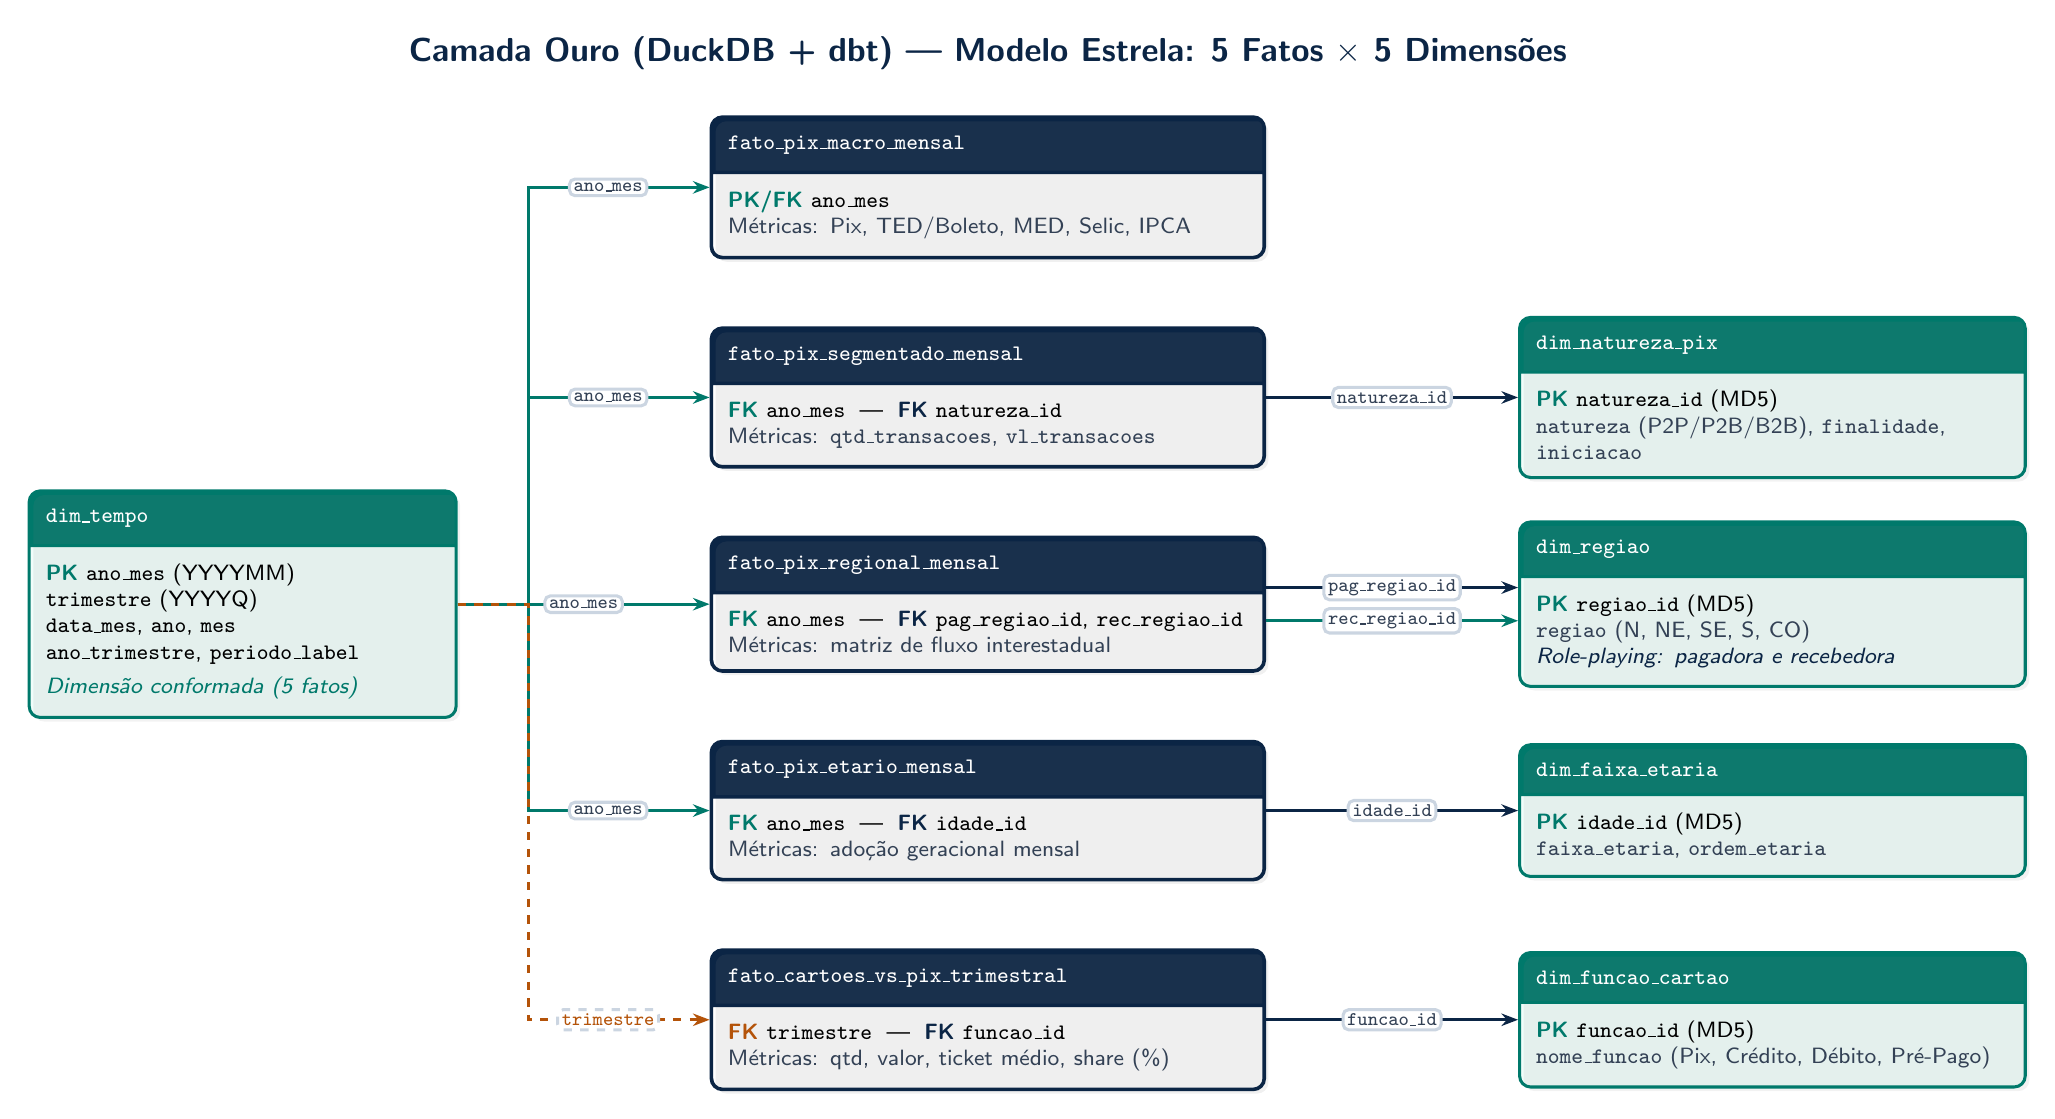
\begin{tikzpicture}[node distance=0.85cm and 2.8cm]

  % --- CENTRO: 5 TABELAS FATO ---
  \node[factbox] (f_macro) {
    \centering\color{white}\bfseries\ttfamily fato\_pix\_macro\_mensal
    \nodepart{second}
    \textbf{\color{teal}PK/FK} \texttt{ano\_mes} \\
    \color{slate} Métricas: Pix, TED/Boleto, MED, Selic, IPCA
  };

  \node[factbox, below=of f_macro] (f_seg) {
    \centering\color{white}\bfseries\ttfamily fato\_pix\_segmentado\_mensal
    \nodepart{second}
    \textbf{\color{teal}FK} \texttt{ano\_mes} \;|\; \textbf{\color{navy}FK} \texttt{natureza\_id} \\
    \color{slate} Métricas: \texttt{qtd\_transacoes}, \texttt{vl\_transacoes}
  };

  \node[factbox, below=of f_seg] (f_reg) {
    \centering\color{white}\bfseries\ttfamily fato\_pix\_regional\_mensal
    \nodepart{second}
    \textbf{\color{teal}FK} \texttt{ano\_mes} \;|\; \textbf{\color{navy}FK} \texttt{pag\_regiao\_id}, \texttt{rec\_regiao\_id} \\
    \color{slate} Métricas: matriz de fluxo interestadual
  };

  \node[factbox, below=of f_reg] (f_eta) {
    \centering\color{white}\bfseries\ttfamily fato\_pix\_etario\_mensal
    \nodepart{second}
    \textbf{\color{teal}FK} \texttt{ano\_mes} \;|\; \textbf{\color{navy}FK} \texttt{idade\_id} \\
    \color{slate} Métricas: adoção geracional mensal
  };

  \node[factbox, below=of f_eta] (f_car) {
    \centering\color{white}\bfseries\ttfamily fato\_cartoes\_vs\_pix\_trimestral
    \nodepart{second}
    \textbf{\color{amber}FK} \texttt{trimestre} \;|\; \textbf{\color{navy}FK} \texttt{funcao\_id} \\
    \color{slate} Métricas: qtd, valor, ticket médio, share (\%)
  };

  % --- ESQUERDA: dim_tempo (CONFORMADA) ---
  \node[dimbox, left=3.2cm of f_reg, text width=5.0cm] (d_tempo) {
    \centering\color{white}\bfseries\ttfamily dim\_tempo
    \nodepart{second}
    \textbf{\color{teal}PK} \texttt{ano\_mes} (YYYYMM) \\
    \texttt{trimestre} (YYYYQ) \\
    \texttt{data\_mes}, \texttt{ano}, \texttt{mes} \\
    \texttt{ano\_trimestre}, \texttt{periodo\_label} \\[3pt]
    \textit{\color{teal}Dimensão conformada (5 fatos)}
  };

  % --- DIREITA: 4 DIMENSOES ESPECIFICAS ---
  \node[dimbox, right=3.2cm of f_seg] (d_nat) {
    \centering\color{white}\bfseries\ttfamily dim\_natureza\_pix
    \nodepart{second}
    \textbf{\color{teal}PK} \texttt{natureza\_id} (MD5) \\
    \color{slate} \texttt{natureza} (P2P/P2B/B2B), \texttt{finalidade}, \texttt{iniciacao}
  };

  \node[dimbox, right=3.2cm of f_reg] (d_reg) {
    \centering\color{white}\bfseries\ttfamily dim\_regiao
    \nodepart{second}
    \textbf{\color{teal}PK} \texttt{regiao\_id} (MD5) \\
    \color{slate} \texttt{regiao} (N, NE, SE, S, CO) \\
    \textit{\color{navy}Role-playing: pagadora e recebedora}
  };

  \node[dimbox, right=3.2cm of f_eta] (d_eta) {
    \centering\color{white}\bfseries\ttfamily dim\_faixa\_etaria
    \nodepart{second}
    \textbf{\color{teal}PK} \texttt{idade\_id} (MD5) \\
    \color{slate} \texttt{faixa\_etaria}, \texttt{ordem\_etaria}
  };

  \node[dimbox, right=3.2cm of f_car] (d_car) {
    \centering\color{white}\bfseries\ttfamily dim\_funcao\_cartao
    \nodepart{second}
    \textbf{\color{teal}PK} \texttt{funcao\_id} (MD5) \\
    \color{slate} \texttt{nome\_funcao} (Pix, Crédito, Débito, Pré-Pago)
  };

  % --- CONEXOES: dim_tempo (1) -> Fatos (N) ---
  \draw[fkarrow] (d_tempo.east) -- ++(0.9,0) |- (f_macro.west)
    node[pos=0.72, fklabel] {ano\_mes};
  \draw[fkarrow] (d_tempo.east) -- ++(0.9,0) |- (f_seg.west)
    node[pos=0.72, fklabel] {ano\_mes};
  \draw[fkarrow] (d_tempo.east) -- (f_reg.west)
    node[midway, fklabel] {ano\_mes};
  \draw[fkarrow] (d_tempo.east) -- ++(0.9,0) |- (f_eta.west)
    node[pos=0.72, fklabel] {ano\_mes};
  \draw[fkamber] (d_tempo.east) -- ++(0.9,0) |- (f_car.west)
    node[pos=0.72, fklabel, text=amber] {trimestre};

  % --- CONEXOES: Fatos (N) -> Dimensoes especificas (1) ---
  \draw[fkfact] (f_seg.east) -- (d_nat.west)
    node[midway, fklabel] {natureza\_id};

  \draw[fkfact] ([yshift=6pt]f_reg.east) -- ([yshift=6pt]d_reg.west)
    node[midway, fklabel] {pag\_regiao\_id};
  \draw[fkarrow] ([yshift=-6pt]f_reg.east) -- ([yshift=-6pt]d_reg.west)
    node[midway, fklabel] {rec\_regiao\_id};

  \draw[fkfact] (f_eta.east) -- (d_eta.west)
    node[midway, fklabel] {idade\_id};

  \draw[fkfact] (f_car.east) -- (d_car.west)
    node[midway, fklabel] {funcao\_id};

  % --- TITULO E RODAPE ---
  \node[above=0.45cm of f_macro, font=\sffamily\bfseries\large, text=navy] {
    Camada Ouro (DuckDB + dbt) --- Modelo Estrela: 5 Fatos $\times$ 5 Dimensões
  };

\end{tikzpicture}
\end{document}
